\documentclass[10pt,a4paper,titlepage]{article}
\usepackage{tabularx}
\usepackage{arydshln}
\usepackage{placeins}
\usepackage{hyperref}
\usepackage{subcaption}
\usepackage[utf8]{inputenc}
\usepackage[T1]{fontenc}
\usepackage{amsmath}
\usepackage{amsthm}
\usepackage{amsfonts}
\usepackage{amssymb}
\usepackage{graphicx}
\usepackage{booktabs}
\usepackage{afterpage}
\usepackage[USenglish]{babel}
\usepackage{mdframed}
\usepackage{todonotes}
\usepackage{threeparttable}
\usepackage{framed}
\usepackage[a4paper, left=1.0cm, right=1.0cm, top=1.5cm, bottom=1.5cm]{geometry}
\setlength{\parindent}{0pt}
\usepackage{xspace}	

\usepackage[makeroom]{cancel}

\newcommand*{\tab}{&}
\newcommand*{\figca}[1]{\caption{#1}}

\usepackage{enumitem}
\setlist{leftmargin=3mm}
\usepackage{refcount}

\usepackage{cases}
\setlength{\parindent}{3em}

\usepackage{chngcntr}
\usepackage{multirow, multicol}
 \usepackage{float}

\counterwithin*{equation}{enumi}
\newcommand{\qr}{QR-Faktorisierung\xspace}
\newcommand{\luf}{LU-Faktorisierung\xspace}
\newcommand{\kui}{Kurven-Interpolation\xspace}
\newcommand{\kua}{Kurven-Approximation\xspace}
\newcommand{\chf}{Cholesky-Faktorisierung\xspace}
\newcommand{\schf}{Sparse \chf}
\usepackage{mathtools}
\DeclarePairedDelimiter\ceil{\lceil}{\rceil}
\usepackage{amsmath,amsfonts,amssymb,amsthm}
\usepackage{mathptmx}
\usepackage{calc}
\usepackage{wasysym}
\begin{document}	

\section{Kurveninterpolation}
\begin{enumerate}[series=b]
	\item \textbf{ Wie kann eine Wurfparabel approximiert werden?}\newline
	\fbox{\parbox[c]{\textwidth}{\luf, \chf,..}}
	\item \textbf{ Wie werden $A$ und $b$ aufgestellt?} \newline
	\fbox{\parbox[c]{\textwidth}{b beinhaltet die Werte $y_i$ der gegebenen Punkte. In $A$ werden die Basisfunktionen gespeichert, also zB. Monome (wie Übung) werden in der ersten Zeile die $x_1^{0...n}$ und in den Spalten $x_{1..n}$ gespeichert. Somit steht in der i-ten Zeile und j-ten Spalte der Eintrag $x_{i+1}^j$.}}
	\item \textbf{ Was ist eine Basisfunktion?} \newline
	\fbox{\parbox[c]{\textwidth}{Eine Basisfunktion beschreibt eine Kurve mit einer endliche Anzahl von Parametern. Die von uns verwendete Basisfunktion ist die Monom-Basis $x^i$.}}
	\item \textbf{ Wie funktioniert \luf und wie löst man das Gleichungssystem?} \newline
	   \fbox{\parbox[c]{\textwidth}{   Faktorisierung von A in untere (L) und obere Dreiecksmatrix (U) mittels Gau{\ss}.\\
	      $	
	      \begin{pmatrix}
		* & * & * & *\\
		* & * & * & *\\
		* & * & * & *\\
		* & * & * & *
	      \end{pmatrix}
	      \rightarrow
	      \begin{pmatrix}
		* & * & * & *\\
		0 & * & * & *\\
		0 & * & * & *\\
		0 & * & * & *
	      \end{pmatrix}
	      \rightarrow
              \dots
              $\\
	      Zum Lösen dann (1) $Ly = b$ und (2) $Ux = y$ lösen.\\
	      Vorwärtssubstitution für (1):\\
              Erstes Element: $y_1 = \frac{b_1}{l_{11}}$ \\
	      $ y_i = \frac{1}{l_{ii}} (b_i - \sum_{j=1}^{i-1} l_{ii}y_{j} )$ für $i = 2, \dots, m$.\\
	      Rückwärts für (2): \\
	      $ x_1 = \frac{y_m}{u_{mm}}$ \\
	      $x_i = \frac{1}{u_{ii}} (y_i - \sum_{j=i+1}^{m} u_{ij}x_j)$ für $i = m-1, \dots, 1$. }}

	\item \textbf{ Wie kann man \luf stabiler machen?}\newline
	\fbox{\parbox[c]{\textwidth}{Pivotisierung der Matrix, mittels Permutationsmatrix.}}
	\item \textbf{ Was ist der Aufwand?} \newline
	\fbox{\parbox[c]{\textwidth}{$PA=LU$: $\frac{2}{3}m^3$ FLOPs.}}
	\item \textbf{ Wann geht der \luf kaputt?} \newline
	\fbox{\parbox[c]{\textwidth}{Die \luf scheitert sobald der Algorithmus versucht eine Division durch 0 durchzuführen. Bsp. Matrix: $\begin{pmatrix}
	0&1\\
	1&1
	\end{pmatrix}$}}
	
\end{enumerate}
\section{Kurvenapproximation}
\begin{enumerate}[resume=b]
	\item \textbf{ Was ist der Unterschied zwischen Approximation und Interpolation?} \newline
	   \fbox{\parbox[c]{\textwidth}{   Polynomgrad bzw. Dimensionen der Matrix $A^{m \times n}$.\\
	      \begin{itemize}
	      \item  $m = n$: $A$ quadratisch, voller Rang, existiert inverse, dann eindeutige Lösung.
              \item  $m > n$: System überbestimmt, nicht exakt lösbar. Approximation.  
              \end{itemize}}}
	\item \textbf{ Wie kann ein überbestimmtes Gleichungssystem approximiert werden?}\newline
	\fbox{\parbox[c]{\textwidth}{Normalengleichung mit folgender \luf, \chf, SVD,..}}
	\item \textbf{ Warum sollte man manchmal ein Polynom kleineren Grades finden?} \newline
	\fbox{\parbox[c]{\textwidth}{Durch ein Polynom mit einem kleineren Grad können verrauschte Daten besser approximiert werden. }}
	\item \textbf{ Was ist der Grad eines Polynomes?}\newline
	\fbox{\parbox[c]{\textwidth}{Der grad eines Polynoms entspricht dessen höchster Potenz}}
	\item \textbf{ Was sind Normalengleichungen und wie sind sie definiert? Welche Dim hat $A^TA$?}\newline
             \fbox{\parbox[c]{\textwidth}{ Erster Teil siehe nächste Frage/Antwort.\\
              $A^TA \in (n \times n)$.}}
	\item \textbf{ Wie leitet man die Normalengleichung her?}\newline
	\fbox{\parbox[c]{\textwidth}{3 Herleitungen, geometrische: \begin{align*}
	Ax=b & \text{ nicht lösbar, da }b \text{ nicht in }range(A)\\
	&\Rightarrow\;y\text{ ist orthognoale Projektion von } b \text{ auf }range(A)\\
	&\Rightarrow r=b-Ax\\
	\|r\|\rightarrow\text{min} &\Leftrightarrow r\perp range(A) = \langle a_1,..,a_n\rangle\\
	&\Leftrightarrow r\perp a_j, j=1,..,n\\
	&\Leftrightarrow a_j^T r=\|a_j\|\cdot\|r\|\cdot cos(a_j,r)=0\\
	&\Leftrightarrow A^Tr=0\\
	&\Leftrightarrow A^T(b-Ax)=0\\
	&\Leftrightarrow A^Tb-A^TAx=0\\
	&\Leftrightarrow A^TAx=A^Tb
	\end{align*}}}
	\item \textbf{ Was ist die 2-Norm?} \newline
	\fbox{\parbox[c]{\textwidth}{$||x||_2=\sqrt{\sum_i x_i^2}$}}
	\item \textbf{ Wann ist eine Matrix symmetrisch positiv definit?}\newline
	\fbox{\parbox[c]{\textwidth}{Eine Matrix is symmetrisch wenn: $A^T=A$ und sie ist positiv definit wenn gilt: $\forall x \neq 0; \; x^T \cdot A \cdot x > 0$.}}
	\item \textbf{ Welcher Löser muss verwendet werden, wenn A nicht quadratisch ist?} \\
          \fbox{\parbox[c]{\textwidth}{    Cholesky, QR oder SVD. Je nach Eigenschaften von A.}}
	\item \textbf{ Was ist der Unterschied zwischen \chf und \qr?}
	\newline
	\fbox{\parbox[c]{\textwidth}{\begin{tabular}{c|c}
		\qr & \chf\\\hline
		eher geometrisch (Basiswechsel) & eher analytisch\\ 
	\end{tabular}\\
	Die QR-Faktorisierung ist besser konditioniert, da sie auf dem geometrischen Ansatz basiert (Konditionierung: $\kappa(A)$). Die \chf verwendet hingegen die Normalgleichungen, welche schlecht konditioniert sind ($\kappa(A^2)$). 
	}}
	
	\item \textbf{ Was ist \chf? Wie funktioniert sie?} \newline
	\fbox{\parbox[c]{\textwidth}{Robuster, effizienter Löser für spd Matrizen. Das Verfahren basiert auf der symmetrischen Gauß-Elimination. Dabei wird die Matrix $A$ in die Faktoren $L$ und $L^T$ zerlegt.  $A=\begin{pmatrix}
	a_{11} & w^T \\
	w & K
	\end{pmatrix}$ \newline
	$A=\begin{pmatrix}	                                                                                                                                                                              \sqrt{a_{11}} & 0 \\
	\frac{w}{\sqrt{a_{11}}} & I
	\end{pmatrix} 
	\begin{pmatrix}	                                                                                                                                                                              1 & 0 \\
	0 & \tilde{L}\tilde{L^T}
	\end{pmatrix}                                                                                                                                                                            
	\begin{pmatrix}	                                                                                                                                                                              \sqrt{a_{11}} & \frac{w^T}{\sqrt{a_{11}}} \\
	0 & I
	\end{pmatrix}   
	=
	\begin{pmatrix}	                                                                                                                                                                              \sqrt{a_{11}} & 0 \\
	\frac{w}{\sqrt{a_{11}}} & \tilde{L}
	\end{pmatrix} 
	\begin{pmatrix}	                                                                                                                                                                              \sqrt{a_{11}} & \frac{w^T}{\sqrt{a_{11}}} \\
	0 & \tilde{L^T}
	\end{pmatrix}  = LL^T$  \newline
	Im Algorithmus wird $L=A$ initialisiert und das obere Dreieck auf $0$ gesetzt. Mit 3 for-Schleifen (aufgrund MatLab Schreibweise) werden dann die Elemente der Spalte wie folgt berechnet: $L(i,j)=L(i,j)-L(i,k)*(L(j,k)/L(k,k))$. Der Wert $x=1/sqrt(L(k,k))$ wird separat berechnet und zum Schluss werden die Elemente der Spalte durch $L(i,k)=L(i,k)*x$ endgültig berechnet.}}
	\item \textbf{ Was ist fill-in und wie kommt es zustande?}\newline
	\fbox{\parbox[c]{\textwidth}{Fill-in beschreibt das eine $a_{ij}=0$ in A ist, aber nach der Faktorisierung mit Cholesky $a_{ij} \neq 0$. Fill-in tritt nur innerhlab des Bandes azf alles Nullen außerhalb des Bandes bleiben erhalten.
		Es ensteht durch die gebildete Differenz $K-ww^T$.}}
	\item \textbf{ Wie funktioniert \qr?} \\
	\fbox{\parbox[c]{\textwidth}{\begin{itemize}
           \item  Erst orthonormale Basis $\{q_1,\dots,q_n\}$ von range$(A)$ konstruieren (Gram-Schmidt)
	   \item  Dann sind Vektoren aus $A$ darstellbar in der gefundenen Basis $\{q_1,\dots,q_n\}$.
           \item  $a_1 = r_{11}q_1, \dots, a_n = r_{1n}q_1 + \dots + r_{nn}q_n$. (Gram-Schmidt liefert auch Koeffizienten $r$)
	   \item in Matrixschreibweise zusammengefasst ergibt sich: $A = QR$
	\end{itemize}
        Für die Lösung eines Least-Squares Problems:
	\begin{itemize}
		\item  QR-Faktorisierung $A=QR$ (siehe oben).
		\item  Berechne $b' = Q^Tb$
		\item  Löse $Rx = b'$ durch Rückwärtssubstitution.
	\end{itemize}}}
	\item \textbf{ Was ist eine orthogonale Projektion?}\newline
	\fbox{\parbox[c]{\textwidth}{Entspricht der Projektion eines Punktes $b$ auf das Bild einer Matrix $A$\\
	beginne mit Projektion von $b$ auf $\langle A\rangle$, mit $\|A\|=1$\\
	$r=b-b'=(I-AA^T)b$, mit $b'=\left(\sum_{i=1}^{k}A_iA_i^T\right)b=\hat{A}\hat{A}^Tb$ mit $\hat{A}\hat{A}^T$ als orthogonale Projektion}}
	\item \textbf{ Wann ist A von vollem Rang?} \newline 
	\fbox{\parbox[c]{\textwidth}{Die Matrix hat den vollen Rang, wenn: $rank ( A ) = n$ $\Leftrightarrow$ $dim ( range ( A )) = n$ $\Leftrightarrow$ $dim < a_1 , . . . , a_n> i = n$ $\Leftrightarrow$ Spalten $a_j$ linear unabhängig $\Leftrightarrow$ $null ( A ) = { 0 }$
	
	}}
	\item \textbf{ Wie ist die Pseudoinverse definiert?}\newline
	\fbox{\parbox[c]{\textwidth}{$A^+ = (A^T A)^{-1} A^T $}}
\end{enumerate}

\section{Konditionierung und finite Differenzen}
\begin{enumerate}[resume=b]
	\item \textbf{ Was ist die Idee der Konditionierung?} \\
        \fbox{\parbox[c]{\textwidth}{Das Problem als Funktion modellieren, welche bei Eingabe $x$ Ausgabe $f(x)$ liefert. Ein Problem ist gut konditioniert, wenn eine kleine Pertubation (Veränderung) in $x$ auch nur eine kleine Pertubation der Ausgabe $f(x)$ bewirkt. Umgekehrt sollte klar sein.}}

	\item \textbf{ Was bedeutete es, wenn ein Problem gut konditioniert ist?}\newline
	\fbox{\parbox[c]{\textwidth}{Ein Problem ist gut konditioniert, wenn eine Störung (Perturbation) in \textbf{x} auch nur eine kleine Störung in \textbf{f(x)} bewirkt. Dabei werden Perturbationen in relativen Änderungsraten gemessen mit: $\frac{\|\delta x\|}{\|x\|}, \;\frac{\|f(x+\delta x)-f(x)\|}{\|f(x)\|}$. }}
	
	\item \textbf{ Was sind finite Differenzen?} \newline
	\fbox{\parbox[c]{\textwidth}{Diskretisierung auf einem regulärem Gitter, wobei die Ableitungen approximiert werden. 
	\begin{enumerate}[itemindent=1em]
		\item Vorwärtsdiff.: $f'[i]\approx \frac{f[i+1]-f[i]}{h}$
		\item Rückwärtsdiff.: $f'[i]\approx \frac{f[i]-f[i-1]}{h}$
		\item  Zentrale Diff.: $f'[i]\approx \frac{f[i+1]-f[i-1]}{2h}$
	\end{enumerate} 
	  
		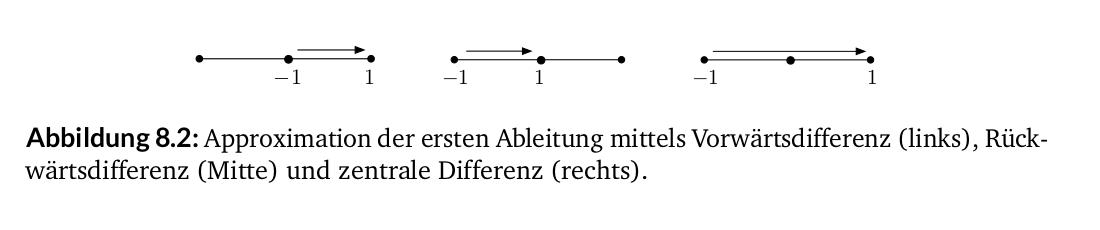
\includegraphics[scale=0.3]{Finitvor}
	
	$\mathop{\!\mathbin\bigtriangleup} u[i,j,t]=\frac{u[i-1,j,t]+u[i+1,j,t]+u[i,j-1,t]+u[i,j+1.t]-4u[i,j,t]}{h^2}$ \\
		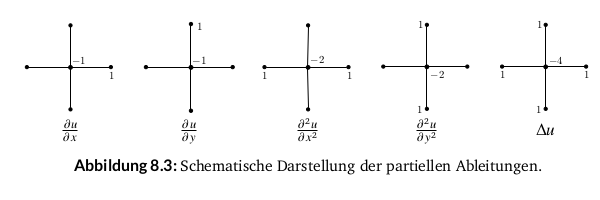
\includegraphics[scale=0.4]{FiniteDiffs}
		

	}}
	
	\item \textbf{ Was bedeuten parabolisch, hyperbolisch und elliptisch?}\newline
	\fbox{\parbox[c]{\textwidth}{Parabolische PDEs beschreiben dynamische Gleichungen die gegen ein statisches Equilibrium konvergieren. Elliptische PDEs beschreiben statische Gleichgewichtszustände. 
		Hyperbolisches PDEs modellieren dynamische Systeme ohne Equilibrium.}}
	\item \textbf{ Was besagt Diskretisierung?} \\
		\fbox{\parbox[c]{\textwidth}{Grundlegende Idee: Kurve (kontinuierlich) mit einer endlichen Zahl von Parametern zu beschreiben. \\
		Dazu Kurve mittels Basisfunktionen $\varphi_j$ und Koeffizienten $f_j$ darstellen: $f(x) = \sum_{j=1}^n f_j\varphi_j(x)$.\\
		Daraus ein LGS zusammenbasteln.}}
	\item \textbf{ Wie lässt sich die erste Ableitung mittels finiter Differenzen approximieren?}\newline
	\fbox{\parbox[c]{\textwidth}{Taylor-Entwicklung erster Ordnung $f(x)+hf'(x)+O(h^2)$ nach $f'(x)$ auflösen\\
	$\Rightarrow f'(x)\approx \frac{f(x+h)-f(x)}{h}$\\
	Wird $f(x)$ diskretisiert mit $f[i]=f(ih)$
	\begin{align*}
	\xRightarrow{\text{Vorwärtsdifferenz}} &f'[i]=\frac{f[i+1]-f[i]}{h}\\
	\xRightarrow{\text{Rückwärtsdifferenz}} &f'[i]=\frac{f[i]-f[i-1]}{h}\\
	\xRightarrow{\text{Zentraldifferenz}} &f'[i]=\frac{f[i+1]-f[i-1]}{2h}
	\end{align*}}}
	\item \textbf{ Was ist der Unterschied zwischen $-\mathop{\!\mathbin\bigtriangleup} u$ und $\mathop{\!\mathbin\bigtriangleup} u$?} \newline
	\fbox{\parbox[c]{\textwidth}{$\mathop{\!\mathbin\bigtriangleup} u[i,j,t]=\frac{u[i-1,j,t]+u[i+1,j,t]+u[i,j-1,t]+u[i,j+1.t]-4u[i,j,t]}{h^2}$: Ausgehend von den Punkten um die Mitte wird davon der mittlere Punkt 4mal abgezogen. \\
	$\mathop{\!\mathbin\bigtriangleup} u[i,j,t]=\frac{4u[i,j,t]-u[i-1,j,t]-u[i+1,j,t]-u[i,j-1,t]-u[i,j+1.t]}{h^2}$: Ausgehen von dem mittleren Punkt, werden die umliegenden Nachbarn abgezogen. \\
	vgl. Abb. Frage 26}}
	
\end{enumerate}
\section{Heat-Equation und Laplace}
\begin{enumerate}[resume=b]
	\item \textbf{ Wie sieht die Heat-Equation aus?}\newline
	\fbox{\parbox[c]{\textwidth}{$ \dot{u}=\mathop{}\!\mathbin\bigtriangleup u$}}
	\item \textbf{ Was besagt $\dot{u} = \mathop{}\!\mathbin\bigtriangleup u$?}\newline
	\fbox{\parbox[c]{\textwidth}{	Siehe vorige Frage.}}
	\item \textbf{ Was ist der explizite/implizit Euler?} (Definition und Vorteile/Nachteile sowie Unterschiede)\newline
	\fbox{\parbox[c]{\textwidth}{Definition vgl. 59\\
	\begin{tabular}{c|c}
		explizit & implizit\\\hline
		\textbf{Vorteile:}&\\
		einfach zu verstehen& verwendet Zeitableitung $\dot{u}$ am nächsten Zeitpunkt $u[t+1]$\\
		einfach zu implementieren &\\
		\textbf{Nachteile:}& \\
		Instabilität bei großen Zeitsprüngen, nicht mehr $\delta t$ konvergiert & stabil für jeden Zeitschritt \\
		Fehler schaukeln stark $\rightarrow$ keine Lösung mehr möglich & höherer Rechenaufwand
	\end{tabular} }}
	
	
	\item \textbf{ Was passiert bei zu hohen Schritten im explizit Euler?}\newline
	\fbox{\parbox[c]{\textwidth}{Es konvergiert nicht mehr, da die Nachbarn einen zu hohen Einfluss auf die Lösung haben. Um das zu berechnen müsste man mehr Nachbarn in Betracht ziehen, da bei zu hohen Zeitschritten auch weit entfernte Nachbarn einen Einfluss auf den betrachteten Punkt haben.}}
	\item \textbf{ Was ist die CFL-Bedingung?})\\
		\fbox{\parbox[c]{\textwidth}{$\delta t \le \frac{h}{||v||}$ mit $||v||$ = Informationsgeschwindigkeit.}}
	\item \textbf{ Wann ist der Gleichgewichtszustand erreicht?}\newline
	\fbox{\parbox[c]{\textwidth}{Der implizite Euler konvergiert immer gegen den statischen Gleichgewichtszustand der Heat-Equation, der durch die Laplace-Equation $\delta u=0$ beschrieben wird. Während der explizite nur bei ausreichend kleinen Zeitschritten konvergiert. }}	
	\item \textbf{ Was beschreiben die Matrizen $U$ und $V$ in der Heat-Equation?} \newline 
	\fbox{\parbox[c]{\textwidth}{In $U$ werden die Höhen der Funktion an jedem Gridpunkt gespeichert. In V wird die Ableitung der Zeit in Bezug auf eine bestimmte Höhe U, also die Geschwindigkeit, gespeichert. }}
	\item \textbf{ Was passiert mit den Randpunkten?} \newline
	\fbox{\parbox[c]{\textwidth}{Die Randpunkte in der Heat-Equation werden nicht verändert.}}
	\item \textbf{ Wie stellt man das lineare Gleichungssystem für die Laplace-Gleichung auf?} \newline
	\fbox{\parbox[c]{\textwidth}{Jeder Punkt im Gitter ist eine Unbekannte die berechnet werden muss, wir haben also bei einem N x N mit Gitter N-2 Unbekannten (Randpunkte verändern sich nicht). Dies führt zu einem $(N-2)^2$ x $(N-2)^2$ Gleichungssystem $-Lu=b$.
		U ist ein Spaltenvektor in dem die neuen Werte U für das Gitter stehen. Die Reihenfolge in der die Gitterpunkte in U stehen führt zu einer Index Abbildung:$u_k=u(i,j)$ mit $k=idx(i,j)=(i-1)+(j-2)\cdot(N-2)$.
		Für die Matrix L gilt: $l_{kk}=4, l_{kl}=-1/h^2$, wenn (\={i},\={j}) Nachbarn von i,j und $l$=idx(\={i},\={j}) sonst $l_{kl}=0$.
	}}
	\item \textbf{ Warum stellt man das lineare Gleichungssystem für den Laplace auf?}\newline
	\fbox{\parbox[c]{\textwidth}{Wir betrachten nur das Gleichgewicht, welches nicht mit expliziter Integration lösbar ist, da es unabhängig von der Zeit ist.}}
	\item \textbf{ Wie unterscheidet sich das Lösen des Gleichungssystems beim Laplace zu den konjugierten?} \newline
	\fbox{\parbox[c]{\textwidth}{Die konjugierten Verfahren lösen dieses iterativ, während bei der Laplace Gleichung genau eine Lösung gefunden wird. Da er unabhängig vom der Zeit ist, kann die explizite Euler Integration nicht angewendet werden. }}
	\item \textbf{ Wie löst man dieses Gl?}\newline
	\fbox{\parbox[c]{\textwidth}{Dieses Gl ist mit der \chf lösbar. Die Zeitkomplexität ist allerdings mit $O(m^3)$ hoch in diesem Fall wodurch die lösungweise durch iterative lösungverfahren besser ist.}}
	\item \textbf{ Welche Eigenschaft hat die Laplace-Matrix?}\\
	\fbox{\parbox[c]{\textwidth}{	$-L$ hat folgende Eigenschaften:
		\begin{itemize}
			\item  Die Matrix ist Sparse: Maximal 5 Einträge pro Zeile, die ungleich null sind.
			\item $-L$ ist symmetrisch.
			\item $-L$ ist positiv definit ($L$ negativ definit).
		\end{itemize}
		}}
\end{enumerate}
\section{Konjugierte Gradienten}
\begin{enumerate}[resume=b]
	\item \textbf{ Wie funktionieren konjugierte Gradienten?}\newline
	\fbox{\parbox[c]{\textwidth}{\begin{align*}
	\text{Beliebige Suchrichtung }p_n \text{ für die Minimierung von } f(x) \text{ zulassen:}\\
	&\Rightarrow x_{n+1}=x_n+\alpha_np_n,\\
	\text{wobei }\alpha_n \text{ ähnlich zum Gradientenabstieg bestimmt werden kann:}\\
	&\frac{\delta}{\delta \alpha_n}f(x_n+\alpha_np_n) = 0\\
	&\Rightarrow \alpha_n=\frac{p_n^Tr_n}{p_n^TAp_n,} \text{ wenn }p_n=-\nabla f(x_n)=r_n \text{ äquiv. zu Gradientenabstieg}
	\end{align*}}}
	\item \textbf{ Wann werden konjugierte Gradienten angewendet?} \newline
	\fbox{\parbox[c]{\textwidth}{Für große Matrizen (m>10000), da sie die Struktur ausnutzen.}}
	\item \textbf{ Was ist $\alpha$?} \newline
	\fbox{\parbox[c]{\textwidth}{$\alpha$ ist die Schrittweite in der wir uns Richtung Lösung bewegen bei einem iterativem Löser. Im Gradientenabstieg ist $\alpha=\frac{r^{T}_{n} r_n}{r^{T}_{n} A r_n}$; in konjugierten Gradienten 
		ist $\alpha=\frac{r^{T}_{n} r_n}{p^{T}_{n} A p_n}$ }}
	\item \textbf{ Was ist die Konvergenz des Gradientenabstiegs?}\\
	\fbox{\parbox[c]{\textwidth}{
	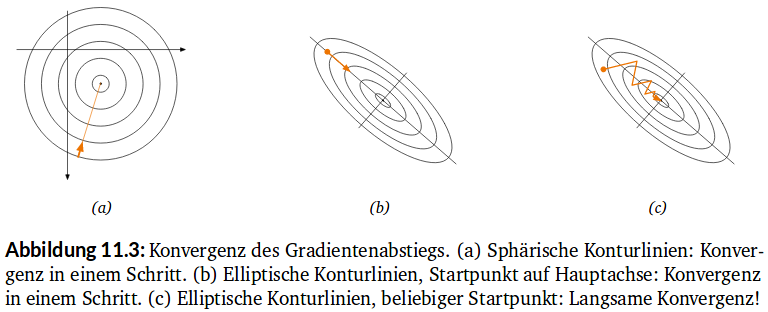
\includegraphics[scale=0.3]{konvergenzgradient}}}
	\item \textbf{ Wie ist der Gradientenabstieg definiert?}\newline
	\fbox{\parbox[c]{\textwidth}{Löse $Ax=b, \text{ mit } A \;s.p.d.$ formuliert als Minimierung $f(x)=\frac{1}{2}x^TAx-b^Tx \rightarrow \text{min}$\\
	$f(x)$ hat ein Minimum, wenn gilt: $0=\nabla f(x)=Ax-b$\\
	minimiere $f(x)$ iterativ, indem bei jedem Schritt von $x_n$ ein Stückchen im Paraboloid heruntergelaufen wird, dies entspricht dem negativen Gradienten $-\nabla f(x)$.\\
	Da $r_n=b-Ax_n=-\nabla f(x)$ folgt $r_n$ als Abstiegsrichtung der n-ten Iteration und $x_{n+1}=x_n+\alpha_nr_n$, mit $\alpha_n=\text{arg min}_\alpha f(x_{n+1})$.}}

	\item \textbf{ Was ist der Unterschied zwischen dem Gradientenabstieg und konjugierten Gradienten?} \newline
	\fbox{\parbox[c]{\textwidth}{Bei dem Gradientenabstieg ist die Schrittweite abhängig von dem Resduum $r_n$. Die konjugierten Gradienten ersetzen $r_n$ durch die Suchrichtung $p_n$, wobei jedes $p_n$ einmalig vorkommt.}}
	\item \textbf{ Was ist eine Datenstruktur für eine dünnbesetzte Matrix?} \newline
	\fbox{\parbox[c]{\textwidth}{Eine einfache Datenstruktur für eine dünnbesetzte Matrix währe das Triple-Format wo alle Einträge $a_{ij} \neq 0$ in einem Tripel (i,j,v) gespeichert werden
		wobei i der Zeilenindex, j der Spaltenindex und v der Wert von $a_{ij}$ ist. Überlicherweise gespeichert als 3 Arrays für jeweils i,j,v.}}
	\item \textbf{ Was sind die Vorteile von konjugierten Gradienten?}\\
	\fbox{\parbox[c]{\textwidth}{\begin{itemize}
		\item  Fehler $ \|e_n\|_A$ nimmt monoton ab.
		\item  Der Algorithmus terminiert nach maximal $m$ Iterationen. 
		\item  Aufwand $O(m^2)$, typischerweise $O(m^{1.5}$.
		\item  Speicheraufwand $O(m)$.
		\item  Algorithmus muss nicht direkt auf Matrix-Einträge zugreifen. Daher Nutzung einer effizienten Datenstruktur für das Matrix-Vektorprodukt $Ap$ möglich.
	\end{itemize}}}
	\item \textbf{ Was ist ein Stopkriterium von konjugierten Gradienten?}\newline
	\fbox{\parbox[c]{\textwidth}{Wenn $A^{n\times n}$ dann kann man nach maximal $n$-Schritte aufhören, ebenso wenn $\beta<\epsilon$.}}
\end{enumerate}

\section{Wave-Equation}
\begin{enumerate}[resume=b]
	\item \textbf{ Wie ist die Wave-Equation definiert? Wie kann man sie als PDE erster Ordnung schreiben?} \newline
	\fbox{\parbox[c]{\textwidth}{$\ddot{u}=c^2 \mathop{\!\mathbin\bigtriangleup}u$. Durch eine Hilfsfunktion $v:=\dot{u}$ kann die Gleichung wie folgt modelliert werden: $\dot{u}=v$ $\dot{v}=c^2\mathop{\!\mathbin\bigtriangleup}u$.}}
	\item \textbf{ Was erfordert eine doppelt so große Wellengeschwindigkeit?} \newline
	\fbox{\parbox[c]{\textwidth}{Eine doppelt so hohe Wellenggeschwindigkeit erfordert einen halb so großem Zeitschritt, damit die explizite Integration nicht instabil wird und weiterhin die CFL bedingung erfüllt. }}
	\item \textbf{ Wie diskretisiert man die PDE's mit finiten Differenzen im Falle der Wave-Equation?} \newline
	\fbox{\parbox[c]{\textwidth}{$u[i,j,t]=u(ih,jh,t\delta t)$, $v[i,j,t]=v(ih,jh,t\delta t)$. Die PDEs hängen num im 2-dim Gitter von Raum und Zeit ab.}}
	\item \textbf{ Wieso müssen Zeitschritte manchmal gesplittet werden?}\newline
	\fbox{\parbox[c]{\textwidth}{Um im expliziten Euler eine große Wellengeschwindigkeit zu berechnen, müssen Zeitschritte gesplittet werden.}}
	\item \textbf{ Welche Randbedingungen sind möglich?}\newline 
	\fbox{\parbox[c]{\textwidth}{\begin{enumerate}[itemindent=1em]
		\item periodisch
		\item  gespiegelt
		\item Null
	\end{enumerate}}}
	\item \textbf{ Was ist der Unterschied zwischen implizit und explizit?} (vlg Heat.) \newline
	\fbox{\parbox[c]{\textwidth}{Explizite Integration berechnet die Werte des nächsten Zeitpunktes $u[t+1]$ aus dem momentaren Werten am Punkt sowie dessen Nachbarn: $u[t+1]=u[t]+\delta t \mathop{}\!\mathbin\bigtriangleup u[t]$.
		Implizite Integration berechnet die Werte des nächsten Zeitpunktes $u[t+1]$ mithilfe des nächsten Zeitpunktes: $u[t+1]=u[t]+\delta t \mathop{}\!\mathbin\bigtriangleup u[t+1]$.
		Zum berechnen von $u[t+1]$ müssen wir das Gleichungssystem:$(I-\delta t \mathop{}\!\mathbin\bigtriangleup )u[t+1]=u[t]$ lösen.}}
	\item \textbf{ Wie sieht das lineare Gleichungssystem im impliziten Fall im Vergleich zum expliziten (Wave Equation) aus?} \\
		\fbox{\parbox[c]{\textwidth}{Im expliziten Fall kann das Gleichungssystem in einem Schritt gelöst werden, da die Gleichungen nicht voneinander abhängen. Im impliziten Fall hängt $v_{t+1}$ aber von $u_{t+1}$ ab und umgekehrt, und muss daher als Gleichungssystem gelöst werden: \\
	\begin{itemize}
		\item $\left( I - \delta t^2 c^2 L \right)v_{t+1} = v_t \delta t c^2Lu_t$.
		\item  Dabei ist $A = \left( I - \delta t^2 c^2 L \right)$, $ x = v_{t+1}$ (gesucht) und
		$b = v_t \delta t c^2Lu_t$
	\end{itemize}}}
\end{enumerate}

\section{Sparse \chf}
\begin{enumerate}[resume=b]
	\item \textbf{ Was ist der Unterschied von Sparse \chf und normaler \chf?}\newline
	\fbox{\parbox[c]{\textwidth}{Für die Sparse Matrix $A$ wird die Spalte $j$ nicht mehr durch all Spalten $k<j$ aus $L$ modifiziert. Die $j$-Spalte wird nur noch durch die Spalten $k$ modifiziert, für die $l_{jk}\neq0$ ist.}}
	\item \textbf{ Was sind fill-ins?} \newline
	\fbox{\parbox[c]{\textwidth}{s. Frage 19}}
	\item \textbf{ Was ist eine Bandmatrix?} \newline
	\fbox{\parbox[c]{\textwidth}{Eine Bandmatrix ist eine dünnbesetzte Matrix deren Nicht-Null-Einträge sich auf ein \glqq Band\grqq \ um die Diagonale der Matrix beschränken, wobei die Bandbreite $\beta(A)$ definiert ist als die maximale Distanz einer Nicht-Null von der Diagonalen der Matrix A.
	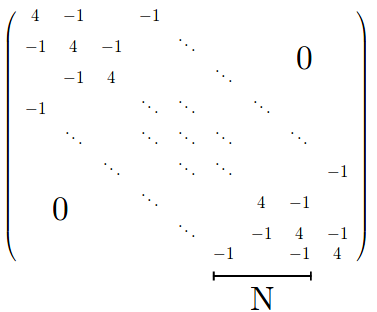
\includegraphics[scale=0.3]{bandmatrix.png}}}
	\item \textbf{ Kommt in der Sparse \chf fill-in vor?}\newline\fbox{\parbox[c]{\textwidth}{Nein.}}
	\item \textbf{ Welche Schritte muss man im Sparse \chf machen?}\newline
	\fbox{\parbox[c]{\textwidth}{Ändere die Reihenfolge der $x_i$ mittels Permutationsmatrix $P$ , so dass $\tilde{x}=Px$\\
	Sortiere analog $A$ um; also $\hat{A}=AP^T$. Da $A$ nun nicht mehr symmetrisch, permutiere nun auch die Zeilen von $A$ und $b$ respektive $\tilde{A}=P\hat{A}=PAP^T$, $\tilde{b}=Pb$.\\ 
	Wende nun Cholesky auf $\tilde{A}\tilde{x}=\tilde{b}$ an.}}
	\item \textbf{ Welche Vorteile hat der Sparse \chf?} \newline
	\fbox{\parbox[c]{\textwidth}{Effizientes, robustes Verfahren für dünn-besetzte Matruzen. Durch eine Umsortierung der Matrix kann es keine fill-ins geben. Durch die Konstruktion von $\tilde{L}$ enthält sie weniger 0en.}}
	\item \textbf{ Was ist die Band-\chf?} \newline
	\fbox{\parbox[c]{\textwidth}{Zunächst lege eine Band-matrix-Datenstruktur für L an. der Speicherverbrauch ist nun $O(mb)$ anstatt $O(m^2)$, wobei b die bandbreite von der Bandmatrix ist. Bei der Berechnung der $l_{ij}$ von L müssen nur Einträge $l_{ij} \in Band(L)$ berücksichtigt werden, da alle anderen einträge null sind. Dies reduziert den Rechenaufwand von $O(m^3)$ auf $O(mb^2)$
		Löse nun $Ly=b$ und $L^Tx=y$ unter Ausnutzung der Bandbegrenzung von L, dies reduziert den aufwand von $O(m^2$ auf $O(mb)$.}}
	
	\item \textbf{ Wieso macht man den Band-\chf und was ist der Vorteil davon?}\newline
	\fbox{\parbox[c]{\textwidth}{Geringerer Speicherplatzverbrauch und schneller (vgl. Frage davor).}}
	\item \textbf{ Was macht der Minimum degree-Algorithmus?}\newline
	\fbox{\parbox[c]{\textwidth}{
	Ziel: Permutation finden, sodass $LL^T=PAP^T$ möglichst wenig fill-in besitzt.\\
	Dazu suche den Knoten $v$ mit den wenigsten Kanten und nummeriere diesen. Des Weiteren verbinde die Nachbarn von $v$ miteinander.}}
\end{enumerate}

\section{Optimierung}
\begin{enumerate}[resume=b]
	
	\item \textbf{  Wie parallelisiert man?}\newline  
	\fbox{\parbox[c]{\textwidth}{Auf einem Prozess mittels SIMD und SSE. Auf mehreren Prozessoren mittel OpenMP (1 Masterthread). Der Code von OpenMP ist: \\
	\# pragma omp parallel
	\\
	id = omp\_get\_thread\_num ();  Welcher Thread ?\\
	int nthreads = omp\_get\_num\_threads () Wieviele? \\
	}}
	\item \textbf{ Welche Kommandozeilen Argumente?} \newline
	\fbox{\parbox[c]{\textwidth}{\begin{itemize}
			\item  -O: schaltet einfache optimierungen ein
			\item  -O3: mehr Optimierungen, insbesondere function inlining
			\item  -Ofast: noch mehr Optimierungen kann aber Ergebnisse verändern!
			\item  --march=native: Aktiviert die passenden AVX/SSE/SSE3 Instruktionen
			\item  -fexpensive-optimizations: Noch mehr Optimierungen
			\item  -funroll-loops Schreibt Schleifen aus.
			\item  -ftree-vectorize: Automatische SSE-Vektorisierung
		\end{itemize}
	}}
	\item \textbf{ Worauf muss man bei Parallelisierung achten?}\newline
	\fbox{\parbox[c]{\textwidth}{Zu beachten ist, dass manche Variablen private gesetzt werden müssen und dass der Speicherzugriff eindeutig sein muss, also Ergebnisse seperat gespeichert werden müssen. }}
	\item \textbf{ Wie kann man Code optimieren?}\newline
	\fbox{\parbox[c]{\textwidth}{Bsp.: Call by Reference, Return by Reference, Inlinen von Funktionen.}}
\end{enumerate}
\end{document}
